\part{Estimation}
\section{Overview}
In this part of the report we will describe and discuss the estimation techniques used in the various sprints of the RentIt project. The sections are structured chronologically, that is in order they where used in the successive sprints. Each described technique will begin with a brief overview of the theory of the technique followed by a reflection on our own experience of employing it.

\section{First techniques: Delphi and Planing Poker}
In our first sprint we used a combination of the two techniques Delphi and Planning Poker.

\subsection{Theory}


The Delphi method is an estimation technique using the size of the collective experience and knowledge from the participating team members.

The technique is broken down into three main sections:
First, each participating team member is given a specification of the given work assignment which is to be carried out, and asked to give an estimate of the time it will take to finish it.
Second, the estimates from all participating team members are gathered and an average of these estimates are calculated. This average is shown to each of the team members.
Third, each team member have the opportunity to reconsider their own estimate relative to the average of the entire team, and, if they so choose, give their own revised estimate.
If a team member decides to change his or hers initial estimate, the whole process is run through once more. This is done until all team members are reasonably satisfied with the collective decision. 
The idea with the above mentioned steps are that since the individual estimates are kept private, there will be no incentive for the team members to begin a discussion about their individual disagreements. In situations like these, it can very often be the person who yells the loudest that gets his or her will, instead of the person who actually presents the most accurate estimate.


Planning Poker is similar to the Delphi technique on several points, including the fact that each team member gives a personal estimate for each individual task and also that it is possible to change your initial estimate later in the process. Where Planning Poker slightly differs from the Delphi method, is that you in Planning Poker get to see the estimate of each individual. If there is an estimation disagreement this can then spur some interesting discussions in order to find common ground. 

From our perspective, this can be conceived as both positive and negative. A positive side is, that you might be able to get a better idea of the actual time needed for the specific subject in question by looking at the estimate from persons who are experienced within the given subject. A negative side is, that there might be people in the team who are oncoming or arrogant in their behaviour, hence they might push the lesser confident people in their direction. 

\subsection{Our experience}


When using the Planning Poker technique, the fact that we could see each others estimates were helpful. There were situations where the estimates were in each end of the scale, and it created some pretty interesting discussions on why this was the case. By having these discussions we very often gained more insight regarding the specific subject, and most of the times each team member could contribute with info the others had not thought about or taken into consideration. It seemed like a good way to get a view from another perspective. We do, however, strongly feel that an important factor here is that the team knows and trusts each other and also can speak freely among each other.
The technique can possibly be very time consuming, but we felt that this were outweighed by the fact that the entire team got a great insight into the individual project tasks, which was derived from the discussions.

The Delphi technique was a similar experience to the Planning Poker technique. It did however distinguish itself on a specific point, namely the fact that it only shows the average of all the estimates. We felt that this approach neither gave us a greater insight into the individual task, nor gave us incentive to discuss the specific task at hand.


\subsubsection{Pros}

Delphi: 
- Only the average of all the estimates are shown which means that nobody will lose face in front of the others
- Each team member has the possibility to change their initial estimate after seeing the average estimate

Planning Poker:
- All estimates are shown which can give each team member a chance to explain their choice
- Each team member has the possibility to change their initial estimate after seeing the average estimate
- Can give a good insight into the individual tasks




\subsubsection{Cons}

Delphi:
- Only the average estimate are shown which creates no direct incentive for discussions

Planning Poker:
- All estimates are shown, which can be negative if some team members try to overrule the others
- Inexperience is a factor that might produce several wrong estimates if it involves the entire team
- Can be time consuming

\section{Second technique: PERT}
\subsection{Theory}

The Program (or Project) Evaluation and Review Technique, commonly known as PERT, is a widely used techniques in use in project planing today. The technique itself includes quite a lot of theory behind structuring tasks and their dependencies with each other, but also includes it own method of estimating. There is an explanation of a very simple version of this method in \cite[p.152]{ProjectManagement_b}, but the following have taken some extended point from \cite{TynerBlain_w} among others\\

The estimations in PERT relies on making multiple estimates for each task, and using that to calculate a weighted average. The estimates consists of a ``best case'', a ``most likely'' and a ``worst case'' estimate. The weighted average is calculated as follows
$\frac{best+4*likely+worst}{6}$
, resulting in a number that is centred around the likely estimate, but can tilt to either sides.\
 
This estimate, or median, is a better guess for how long a task will take to fulfil. But there is still a deviation. We here talk about the standard deviation, which we calculate as 
$\frac{worst-best}{6}$
, and represents the uncertainty in the estimate. With this, we can interpret our median of the original three estimates as a probability, how likely a task is to finish within a time frame. \
This is done by distributing the probability across the time frame, some how resembling of a \textit{normal distribution}. Cumulating between two time estimates, can then give you the probability of how likely the task is to finish sometime within the timespan of the two estimates [See fig. something]. \
\begin{center}
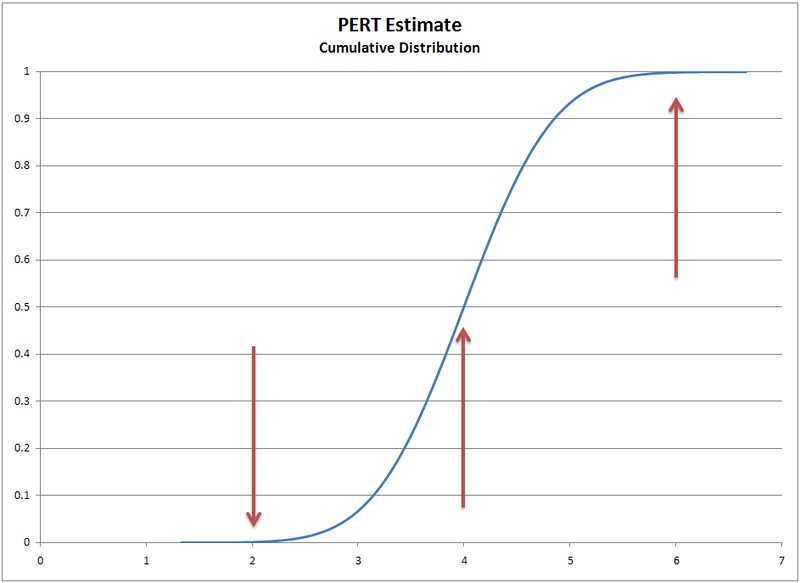
\includegraphics[scale=0.5]{PERTDistribution.png} 
\
\textit{There is nearly a hundret percent chance the task will finish sometime between 2 and 6 hours}
\end{center}

Choosing how to do this distribution is though a bigger mathematical and statistical problem, which we will not discuss here, since it is out of scope.

For our purpose some general distribution for this is though used in many projects and gives a pretty good picture of how these estimates can be used. These are taken from [Wiki: Three-Point Estimation]\
\begin{itemize}

\item The PERT estimate = 50 \% probability.
\item Pert estimate +/- standard deviation = 68 \% probability.
\item Pert estimate +/- 2 x standard deviation = 95 \% probability.
\item Pert estimate +/- 3 x standard deviation = 99.7 \% probability.
\end{itemize}
An example would be that the three estimates of 3/5/10 hours would give you a median of 5.5, and a standard deviation of 1.17. So there is a 50 \% chance the task will be finished within 5.5 hours, but adding the standard deviation there is a 99.5 \% chance the task is finished in 1.9-9.1 hours.\
The PERT-estimate and deviations no longer directly reflects the original estimate, and have drifted somewhat, but these new numbers, derived from a probability, should end up being truer than what the team originally estimated. \\



\subsection{Our experience}
Utilizing this technique was a new experience for us, and changed the way we had formerly viewed estimation. The very scientific approach, utilizing mathematical analysis to achieve our results, help us to distance ourself from the different tasks, and sped up the process of estimation. The feeling that our guesses would not be the precise and final estimate, drove us to discuss less in terms of how much time we thought would be used for a task, and more in the lines of how uncertain we were about what would be needed for the task to be successfully finished within the deadline. \\

Beginning the sprint and starting implementation and completing tasks, we did though get a bit detached from the estimates, because of the very "floating" nature for the numbers, due to them being probabilities instead of actual estimates. This detachment combined with the fact that during this sprint a lot of unexpected work arose from our international collaboration, made the accuracy of these estimates hard to judge. \\

\subsubsection{Pros}
\begin{itemize}
\item The time it takes to make the estimates is reduced by calculating the deviations mathematically instead of basing it around a discussion. 
\item Giving a variable and broad intervals of estimation helps to visualise the estimates as part of a process, not just some arbitrary number.
\item Having a deviation to go by makes it easier to quickly spot if a task is within an acceptable range from the median estimate, not having to judge it "by eye".

\end{itemize}

\subsubsection{Cons}
\begin{itemize}
\item Detachment from the estimates, seeing them as probabilities, makes it harder to follow them during the implementation process.
\item When making the estimates it can be tempting to not think each sub-estimate through, as it will be "hidden" behind the calculated estimate.

\end{itemize}

To conclude, our experience with PERT was mixed. The ease of estimation is one of the biggest pros, and the step back from just viewing estimates as simple numbers. But for our scope, this detachment from the estimates proved a bit to much.

\section{Third technique: Direct estimation based on project breakdown}
\subsection{Theory}
The direct estimation technique can be used in situations where a project has been broken down into smaller tasks. After a detailed list of tasks has been created, one or several estimators will give their assessment on the effort needed to perform each task. The total effort needed for the entire project is then calculated by summarizing all the individual task estimates.
The technique is a good approach in the developing plans for sub-stages of a project, like an upcoming sprint while it is not that useful on the sprints that lies further ahead in the process. This is the main reason why we chose to implement it in our final sprint, since all remaining tasks were known and easy to estimate.


\subsection{Our experience}
Our experience with the direct estimation technique has been a little vague. We did not feel that it contributed with anything that was not already implemented in the previous tested methods or techniques. 

\subsubsection{Pros}
- If the estimators possess a decent amount of knowledge and experience within the subjects of the tasks, very reliable estimates can be given. 

\subsubsection{Cons}
- This technique can be difficult to use in the beginning phase of a project, since here it is not always that all necessary information is available.
- The direct estimation technique can be very time consuming, and thereby costly, to use.
- If the estimators are inexperienced the time and resources used on estimation can possibly be wasted


\section{Comparison and results}

In this section we will compare the efficiency of the tested estimation techniques against the deadlines they help set, and discuss the reasons, conditions and constraints that have led to these different outcomes.

\subsection{Precision of estimation}
The optimal way to compare these techniques, would have been to estimate the exact same tasks, for the exact same project, on the exact same day. The we could just have seen what method gave the most precise estimate. Because of time constraint, as the project we estimated had a different purpose and goal than this report, this was not possible. Therefore we can not just do a side-by-side comparison of the three methods because we have applied them to somewhat different parts of the project. We will still try to evaluate the precision of each technique, but also how it impacted the process of estimating, and the effects later in the implementation of the tasks that have been estimated. \



Delphi/Planning Poker

The technique used to estimate the tasks for our first sprint gave us some valuable info about each of the specific tasks chosen. Whenever we had an estimation disagreement then the following discussion led to a greater insight about the task in question. This meant that each team member obtained a good overview of the project in general, which was helpful both during the initial as well as the following sprints.

The precision of our estimates were pretty decent compared to the actual results. However, there were some complications regarding the collaboration with the Singaporeans. We had a situation during the first sprint where we had to complete some tasks that was not a part of the sprint to begin with, due to an urgent request from their side. This meant that we basically completed a weeks worth of tasks during a single day. But since not all tasks had been initially estimated and included in the sprint it somewhat made it difficult to give a solid overview of the efficiency of the estimation technique. 



When looking at the precision of the estimates, the PERT estimations have the positive point, of already having a buffer from the start, given by the calculated uncertainty. For our second sprint, when we applied PERT for our estimation, we had 100.5 hours of available work time for our team. We made our estimates, and decided on tasks representing 104.5 hours of work, with the buffer telling us that we should definitely be done within between 91.5 and 118 hours. So from the start, we knew we had a possibility of going over time. \

But even with this buffer, the estimates were still of, and at the end of the sprint we had more than 30 hours of work left. About double the deviation we had already applied. So in this aspect PERT did not fair well. This could very well be connected to the fact, that we did not get in to discussing the tasks very much, so especially some of the bigger tasks went proportionally a lot over the estimates. \

The process of estimating itself was though one of the quickest of the project. We got a good feeling for the estimates as probabilities, but we might have lacked some of the grounding in the tasks themselves. This carried over to the phase of implementing the tasks, making it hard to re-estimate how much time was left, as task and estimate was not that connected any more. A different experience all together. \\


Our third sprint was centered around the technique "Direct estimation based on project breakdown". The experience here was very similar to the one we had with PP where the project was broken down into smaller tasks before an estimate was placed by each team member. The main difference that we found, is that the technique does not directly encourage you to discuss the estimates as much as the PP technique, even though it is sort of implied in order to find common ground.



From the events that happened during our international collaboration, a few features was pushed to the next sprint, and was hence estimated both with Planning Poker and PERT. As to not mix the results of the processes up, we did not take the estimates from PP into consideration during the PERT technique. This resulted in two quite different estimates, but they mirror many of our observations.\

The Planning Poker ended up with five sub-tasks for the feature of uploading media, adding up to a total of 10 hours of work. When it came to PERT we had some experience from the first sprint, and our estimates were a bit more cautious. We made it as just one task, and estimated it would take 18 hours with 6 hours of uncertainty.\

In the end the feature of uploading a video took about 20 hours to implement. Here the PERT estimate were closest and actually within the error margin. But considering what the sub-tasks from PP consisted of, 10 hours is not far of, seeing as there is no sub-task for sending the video over the network, which ended up being the biggest hurdle in this. This proves that the breaking down of the task, and discussing them during the PP estimations, produced solid tasks and estimates, that was thought through. But it also shows, that if enough information and knowledge is at hand, bigger tasks can sufficiently be estimated with PERT, giving a reasonable margin of error. \


\begin{itemize}
\item How do different estimation techniques affect the teams' ability to meet project deadlines?

\item How does the working conditions influence the precision and usefulness of the various estimation techniques?	

\item Is one estimation technique more appropriate than others in a project of size and scope similar to a 4 month university project?
\end{itemize}
















